\section{Issues}
\label{section: methodology - issues}

Some general issues that were encountered during the creation of this thesis will be discussed here.
These issues will have affected multiple of our attempted approaches.

\subsection{Cascading Replay Offset}
\label{sub-section: methodology - issues - cascading replay offset}

\begin{wrapfigure}{l}{0.35\textwidth}
    \caption{Issues with pre-configuration replays}
    \centering
    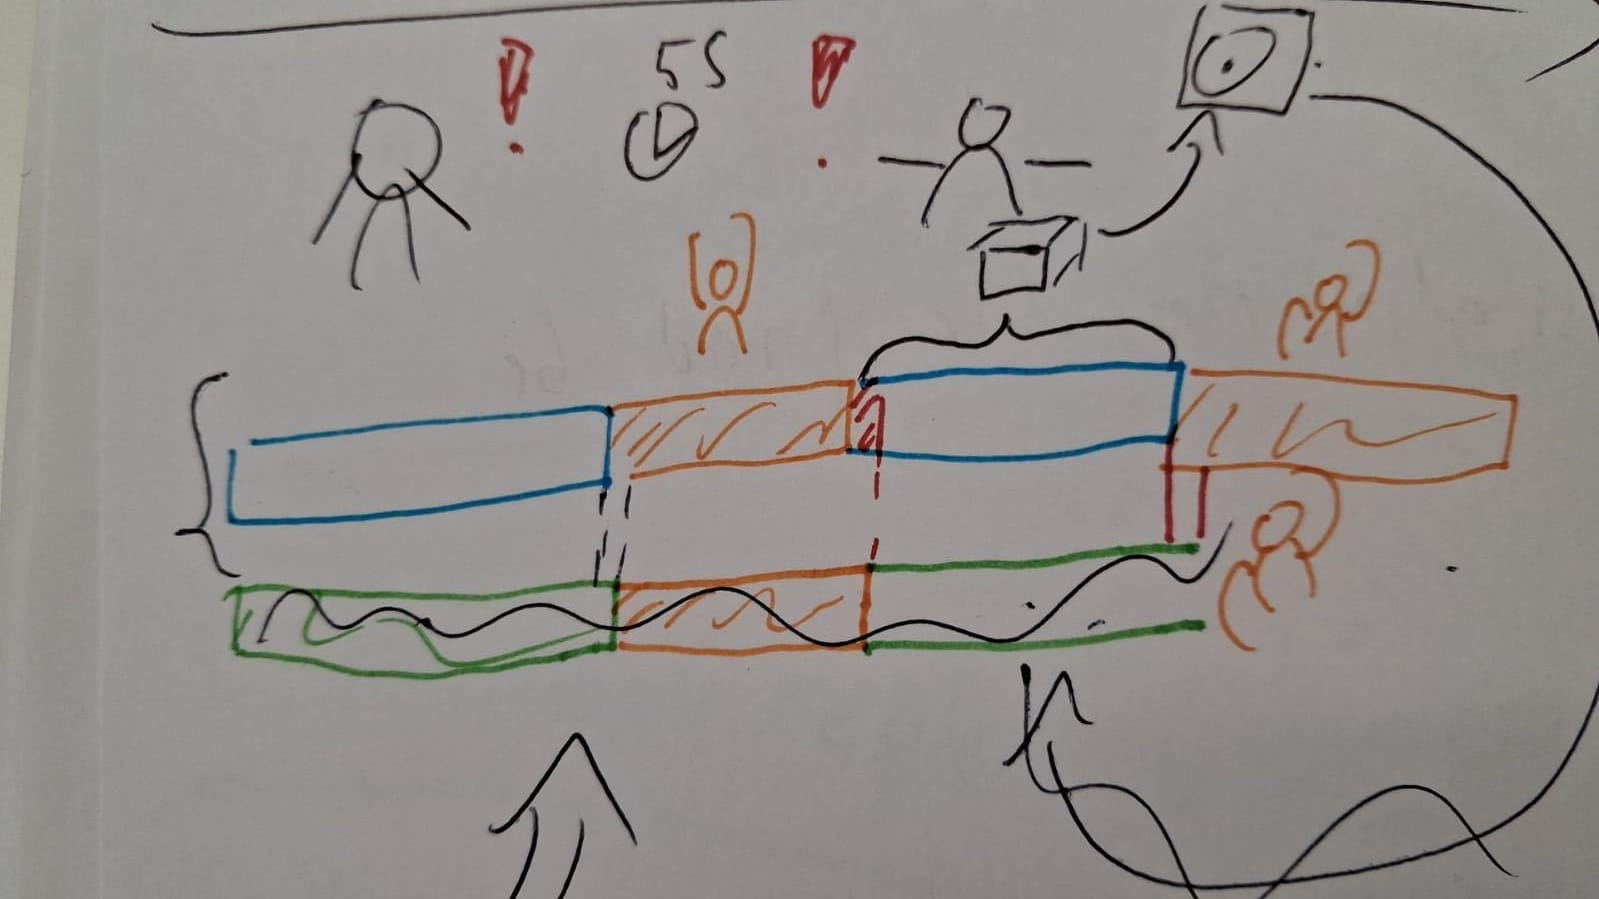
\includegraphics[width=0.35\textwidth]{figures/pre-configuration replay issue.png}
    \label{fig: pre-config issue}
\end{wrapfigure}

During the creation of the filters some issues arose, some of these issues required a rethinking/rewriting of the code to solve, while others required a new system to circumvent their problems.
One such issue was the fact that the \textit{pre-configuration} (see \cref{Section: methodology - preconfiguration}) would not initialize properly during replay.
This issue occurred as some frames may come milliseconds later in the replay then in the origional live recording, this could then lead to the next configuration step getting stuck, as it did not receive enough points in time, since the user was prompted that that configuration step was finished they may have moved their arms into a problematic position (away from the config position), see \cref{fig: pre-config issue}.
\\
The two sollutions to this issue would be: 
\begin{enumerate}
    \item To embed markers of the start and end of each config step into the mmwave data. 
    \item To save all datapoints recorded during pre-configuration and save those seperately.
\end{enumerate}
The first option forces you to save this information in your raw pointcloud recording, which is not optimal, though possible. 
The second options requires you to write an extra file, and read an extra file in during replay, however, it also offers a few general benefits.
You will not have to wait for the pre-configuration anymore when replaying a recording of the mmwave.
You can change the pre-configuration algorithm somewhat without breaking the code.

With these considerations in mind the second sollution was chosen, since it provides some extra benefits while both solutions are roughly an equal amount of work to implement

\subsection{Skewed Data}
\label{sub-section: methodology - issues - skewed data}
I want to discuss the consistent data skew (more data on one side then the other), why this was such a big issue, and how I worked around it

One issue I often encountered was the data being skewed to the cameras right. Meaning, if I am standing in front of the camera, and perform the same action with my right and left hand, I get significantly more points on my left side (the cameras right view) then on my right side.

\subsection{Noisy Data}
\label{sub-section: methodology - issues - noisy data}
Discuss the general way we encountered noise, the persistence of it, and the fact that it was often streaked and single frame only.
Also discuss that the noise level was in part dependent on the room we where in, meaning that one filter tuning would never work for multiple rooms at the same time

Our FMCW had a problem where the data often had noise streaks in the point cloud, this needed to be filtered out, or would throw off many an algorithm.

I am still using a kind of strnage firmware (from one of my earlier tests) this may not produce the best pointclouds, should be mentioned, maybe in discussions though.


